\documentclass[]{article}
\usepackage{graphicx}
\usepackage{pdfpages}
%opening
\title{Appunti di Automi e Linguaggi Formali}
\author{Nicola Baesso}

\begin{document}

	\maketitle
	
	\newpage
	\tableofcontents
	\newpage
	
	\textbf{Disclaimer}
	\newline
	\newline
	Questi appunti sono una raccolta parziale delle spiegazioni del prof. Bresolin, e sono state scritte con la gioia di poterle portare ai parziali e all'esame. Si consiglia comunque di utilizzare solo come eventuale ripasso e non come testo di studio.\\
	Il materiale utilizzato sono: slide del docente, soluzioni fornite dal docente e dal tutor.
	\newpage
	\section{Introduzione}
		\subsection{Definizioni utili alla comprensione}
			Per questo corso, ci si avvarrà di alcune definizioni riportate in seguito, utili per una migliore comprensione della materia.
			\subsubsection{Algoritmi e Problemi}
				Un problema è definito da 3 (tre) caratteristiche specifiche: l'insieme dei possibili input, l'insieme dei possibili output e la relazione che collega questi due insiemi.
				\newline
				Un algoritmo è una procedura meccanica che, eseguendo delle computazioni eseguibili da un calcolatore, risolve un determinato problema se per ogni input si ferma dopo un numero finito di passaggi e produce un output corretto.
				\newline Inoltre è composto da una complessità temporale, che indica il tempo di esecuzione, e una complessità spaziale, che indica la quantità di memoria utilizzata. Entrambe queste misure sono dipendenti dalla dimensione dell'input.
			\subsubsection{Linguaggi formali}
				Un linguaggio formale può essere definito come un'astrazione del concetto di problema. 
				\newline
				Infatti, un problema può essere espresso sia come un insieme di stringhe (che da qui in avanti indicheremo con Linguaggio), con soluzioni che indicano se una stringa è presente nel Linguaggio o meno, oppure come una trasformazione tra vari Linguaggi, dove la soluzione trasforma una stringa di input in una stringa di output.
				\newline
				Quindi, ogni processo computazionale può essere ridotto ad una determinazione dell'appartenenza ad un insieme di stringhe, oppure essere ridotto ad una mappatura tra insiemi di stringhe.
			\subsubsection{Automi}
				Un automa è un dispositivo matematico (inteso in forma astratta) che può determinare l'appartenenza di una stringa ad un Linguaggio e può trasformare una stringa in una seconda stringa. Possiede ogni aspetto di un computer, poichè dato un input provvede a fornire un output, è dotato di memoria e ha la capacità di prendere delle decisioni.
				\newline
				La memoria per un automa è fondamentale. Sostanzialmente esistono automi a memoria finita e automi a memoria infinita, quest'ultimi con accesso limitato e non.
				\newline Chiaramente si hanno vari tipi di automi, ognuno di questi adatti ad una determinata classe di linguaggi, dove vengono differenziati per quantità di memoria e per il tipo di accesso ad essa.
			\subsubsection{Alfabeto e Linguaggio}
				Esattamente come nel caso del linguaggio naturale, un alfabeto è un insieme finito e non vuoto di simboli, ed è indicato con il simbolo $\Sigma$. Da esso si ha la stringa, ovvero una sequenza finita di simboli presi da un alfabeto. Inoltre, si definisce come stringa vuota la stringa senza alcun simbolo preso dall'alfabeto, e si indica con il simbolo $\varepsilon$. Infine la lunghezza di una stringa indica il numero di simboli presenti nella stringa, indicandola con \textbar w\textbar, con w una stringa qualsiasi .
				\newline
				\newline
				\textbf{Esempio}
				Si consideri il codice binario, composto da 0 ed 1. Allora definiremo l'alfabeto come $\Sigma$=\{0,1\}, una stringa valida come w=010110, e in questo particolare caso \textbar w\textbar=6.
				\newline
				\newline
				La potenza di un alfabeto, espressa come $\Sigma$$^k$ con k$\textgreater$0, esprime l'insieme delle stringhe composte da simboli dell'alfabeto di lunghezza k. L'espressione $\Sigma$$^*$ indica l'insieme di tutte le stringhe sull'alfabeto.
				\newline
				\newline
				\textbf{Esempio}
				Consideriamo nuovamente il codice binario. Per 0$\textless$k$\textless$2 (inclusi) si ha \newline
				$\Sigma$$^0$=$\varepsilon$ (la stringa vuota) \newline
				$\Sigma$$^1$=\{0,1\}\newline
				$\Sigma$$^2$=\{00,01,10,11\} \newline
				E così per ogni k positivo. Mentre $\Sigma$$^*$=$\Sigma$$^0$ $\cup$ $\Sigma$$^1$ $\cup$ $\Sigma$$^2$ \ldots \newline \newline 
				Quindi la potenza di un alfabeto crea a sua volta un alfabeto, con stringhe di lunghezza k, e tale alfabeto è composto da 2$^k$ stringhe. 
				\newline
				\newline
				Un linguaggio L è un sottoinsieme dell'insieme di tutte le stringhe dell'alfabeto. In simboli: L $\subseteq$ $\Sigma$$^*$ per un certo $\Sigma$.
			\subsubsection{Operazioni sui linguaggi}
				Definiamo le operazioni che si possono fare sui linguaggi: \newline \\
				-Unione: L $\cup$ M=\{w : w $\in$ L oppure w $\in$ M\}\\
				-Intersezione: L $\cap$ M=\{w : w $\in$ L e w $\in$ M\}\\
				-Concatenazione: L.M=\{uv : u $\in$ L e v $\in $M\}\\
				-Complemento: $\overline{L}$=\{w : w $\notin$ L\}\\
				-Chiusura di Kleene (o Star): L$^*$=\{w1,w2,...wk : k $\ge$ 0 e ogni wi $\in$ L\}\\\\
				Tutte questa operazioni godono (e ci fanno godere) della proprietà di chiusura. In altre parole, se L e M sono linguaggi regolari, allora anche L $\cup$ M, L $\cap$ M, L.M, $\overline{L}$ e L$^*$ sono linguaggi regolari.\\\\
				\textbf{Importante!} Nelle prossime righe si parleranno di DFA, funzioni di transizioni e quant'altro. Se non si ha la più pallida idea di cosa significhino queste espressioni, v'invito a passare per la sezione DFA del seguente file, e successivamente ritornare sull'esempio che segue.
				\\\\
				\textbf{Esempio} Vogliamo (in realtà no, ma ci serve) dimostrare che la proprietà di chiusura vale per l'intersezione (dimostriamo la chiusura per intersezione).\\
				Partiamo dal fatto (che vedremo in dettaglio più avanti) che, essendo L e M linguaggi regolari, esiste un DFA che accetta L e un DFA che accetta M. Quindi, essendo anche L $\cap$ M un linguaggio regolare, possiamo costruire un automa (più precisamente, un DFA) rappresentativo del linguaggio. In particolare, questo automa simula Al che Am in parallelo, e accetta una parola $\Leftrightarrow$ tale parola è accettata sia da Al che da Am.\\
				La funzione di transizione dell'automa è formata da (p,q) $\rightarrow$ (s,t), con p $\rightarrow$ s funzione di transizione di Al, e q $\rightarrow$ t funzione di transizione di Am.\\
				L'automa accetta una parola solo se Al e Am sono entrambi in uno stato finale. In altre parole, con p stato di Al e q stato di Am, l'automa accetta una parola solo se (p,q) è una coppia di stati finali. Formalmente:\\\\
				AL$\cap$M=(Ql $\times$ Qm, $\Sigma$, $\delta$L$\cap$M, (ql,qm), Fl $\times$ Fm)\\
				dove il simbolo $\times$ è il prodotto cartesiano.\\\\
				L'esempio prende in considerazione il linguaggio L$\cap$M, ma il concetto della costruzione dell'automa è valido anche per dimostrare la proprietà di chiusura nelle altre operazioni.
				
	\section{DFA, NFA, espressioni e Linguaggi (non) regolari}
		Dopo aver appreso le definizioni necessarie, andiamo a scoprire in questa sezione i primi automi (DFA ed NFA), cosa sono le espressioni regolari e cosa sono i Linguaggi non Regolari.
		\subsection{DFA}
			Gli Automi a Stati Finiti (in Inglese Deterministic Finite Automation, abbreviato in DFA) sono la forma più semplice di automa e dispongono di una quantità finita di memoria.
			Tali automi accettano una parola nel linguaggio unicamente se è in uno stato terminale.
			\newline
			\newline
			\textbf{Esempio}
			Trovare ogni parola nel linguaggio binario che sia composta da un numero pari di 1.\newline
			Per creare questro DFA, abbiamo bisogno di due stati:\newline
			-Il primo sarà lo stato con il numero pari di 1. Tale stato sarà sia iniziale che terminale (e quindi accetterà la stringa).\newline
			-Il secondo sarà lo stato nel quale si ha un numero dispari di 1. In tale stato l'automa non accetterà la stringa.\newline
			Nel caso s'incontri uno 0, si deve rimanere nello stato attuale.\newline
			Segue il diagramma di transizione dell'automa, fatto con JFlap:
			\newline
			\begin{center}
				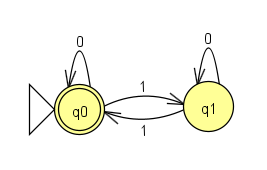
\includegraphics{DFA1.png}
			\end{center}
			Si noti, nel esempio, che ogni stato esegue una transizione \textbf{per ogni simbolo nel linguaggio}. Inoltre, quello che fa l'automa è semplicemente "contare" quante cifre di 1 sono presenti, accettando la stringa solo quando questa cifra è pari.\newline
			In generale, possiamo dire che un DFA utilizza un numero di stati per "contare" ad un determinato scopo, ed ha una transizione per ogni simbolo del linguaggio che deve analizzare.\newline
			\newline
			In maniera formale, un DFA si definisce con A=(Q,$\Sigma$,$\delta$,q0,F), dove Q è un insieme finito di stati, $\Sigma$ è un alfabeto finito (rappresenta i simboli dati in input al DFA), $\delta$ è una funzione di transizione ((q,a)$\mapsto$ q'), q0 è lo stato iniziale (e logicamente è nell'insieme di tutti gli stati dell'automa. In simboli: q0 $\in$ Q), e F è un insieme di stati finali (ovvero gli stati dove l'automa accetta la stringa, in simboli F $\subseteq$ Q).
			\newline
			\newline
			Come già visto nell'esempio, un DFA può essere graficamente rappresentato con cerchi, ad indicare gli stati, e con frecce, ad indicarne le transizioni. Però un DFA può essere rappresentato anche tramite una tabella, chiamata tabella di transizione.
			\newline
			\newline
			\textbf{Esempio} Riprendiamo l'esempio precedente. \newline
			Abbiamo già espresso l'automa che accetta ogni linguaggio con un numero pari di 1 come diagramma di transizione. Ora rappresentiamolo come tabella di transizione. \newline
			Per fare ciò, partiamo dallo stato iniziale, nel nostro caso q0, e ci segniamo le sue transizioni: se si ha uno 0, l'automa resta in q0, mentre se si ha un 1 l'automa va nello stato q1. Per q1 si fa la stessa cosa: se si ha uno 0, l'automa resta in q1, mentre con un 1 l'automa va (in questo caso, ritorna) in q0.\newline
			Di seguito, in forma tabellare, quel che ci siamo appena detti: \newline
			\begin{center}
				\begin{tabular}{c|c|c}
					 &0&1 \\
					 \hline
					$\rightarrow$ q0* &q0*&q1 \\
					q1&q1&q0*
				\end{tabular}
			\end{center}
			Come si nota dall'esempio, nella tabella di transizione si segna con una freccia lo stato iniziale dell'automa, e con un asterisco lo stato finale dell'automa stesso (che nel nostro esempio coincide con lo stato iniziale, ma non è sempre così).\newline
			\textbf{Importante!} Un DFA accetta una parola w se la sua computazione accetta w, ovvero l'automa termina in uno stato finale. Inoltre, se il DFA accetta w, allora w appartiene ad un linguaggio regolare. \newline
			Più formalmente, si indica con L(A)=\{w $\in$ $\Sigma$$^*$  \textbar A accetta w\} il linguaggio accettato, che è un linguaggio regolare.
		\subsection{NFA}
			Gli Automi a Stati Finiti non Deterministici (in inglese Nondeterministic Finite Automation, abbreviato in NFA) sono una forma di automi a stati finiti, che è utilizzato in contesti dove "contare" non è semplice, quindi si lascia spazio al non-determinismo. \newline
			\textbf{Esempio} Costruire un NFA che riconosca la parola che, sull'alfabeto \{a,b,c\}, non sia composto da tutti i simboli. \newline
			Per questo esempio, usare un DFA risulterebbe alquanto complesso, quindi ci avvarremo di un NFA per semplicità. Infatti, ci saranno sufficienti 4 stati e 6 transizioni in tutto. Di seguito troviamo sia tabella che diagramma di transizione per il seguente NFA:\newline
			\begin{center}
				\begin{tabular}{c|c|c|c}
					&a&b&c \\
					\hline
					$\rightarrow$ q0 &\{q1,q3\}*&\{q1,q2\}*&\{q2,q3\}* \\
					\{q1,q2\}* &q1*&\{q1,q2\}*&q2* \\
					\{q1,q3\}* &\{q1,q3\}*&q1*&q3* \\
					\{q2,q3\}* &q3*&q2*&\{q2,q3\}* \\
					q1* &q1*&q1*&$\emptyset$ \\
					q2* &$\emptyset$&q2*&q2* \\
					q3* &q3*&$\emptyset$&q3* \\
				\end{tabular}
			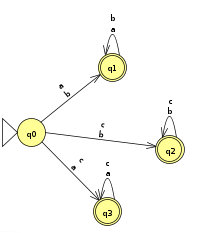
\includegraphics{NFA1.png}
			\end{center}
			Esattamente come prima, nella tabella rappresentiamo lo stato iniziale con una freccia e con un asterisco rappresentiamo lo stato finale. Generalmente, può capitare che la tabella di transizione può essere "smagrita" ovvero che la tabella completa contiene transizioni a stati mai attraversati dall'automa (non è il caso dell'esempio), e quindi possono essere rimossi. Notiamo però che gli stati inclusi nella tabella non sono semplicemente solo gli stati semplici ma includo anche dei "gruppi" di stati, essendo le transizioni dirette in più stati (grazie al non-determinismo).\newline
			Formalizziamo: un NFA NA è descritto con NA=(Q,$\Sigma$,$\delta$,q0,F), con l'unica differenza (rispetto ai DFA) che la funzione di transizione restituisce un sottoinsieme di Q. \newline
			\textbf{Importante!} Un NFA, a differenza di un DFA, può non arrivare alla fine della computazione ed interrompersi prima (come si nota bene dalle tabelle di transizioni), e quindi accetta una parola w se almeno una sua computazione accetta w, ovvero l'automa termina, in almeno una delle sue computazioni, in uno stato finale. Esattamente come nel DFA, se l'NFA accetta w, allora w appartiene ad un linguaggio regolare (la formalizzazione è la stessa).
			\subsubsection{$\varepsilon$-NFA}
				Gli $\varepsilon$-NFA sono NFA che utilizzano le $\varepsilon$-transizioni, ovvero utilizza transizioni che \textbf{non consumano il carattere}, quindi l'automa passa allo stato successivo mantenendo la stringa come prima. \newline
				\textbf{Esempio} Costruire un $\varepsilon$-NFA che accetti numeri decimali, riconoscendo il segno (opzionale),una stringa di decimali, un punto e un altra stringa di decimali, tenendo conto che una delle stringhe di decimali non può essere vuota. \newline
				In questo caso, usare un NFA semplice non è una buona idea, poichè non ci permette di dare opzionalità per quanto riguarda il segno. Inoltre non ci farebbe finire in uno stato finale al termine della lettura dei decimali. Di seguito troviamo sia tabella che diagramma di transizione per il seguente $\varepsilon$-NFA:\newline
				\begin{center}
					\begin{tabular}{c|c|c|c|c}
						&$\varepsilon$&+,-&.&0,..,9 \\
						\hline
						$\rightarrow$ q0 &q1&q1&$\emptyset$&$\emptyset$ \\
						q1 &$\emptyset$&$\emptyset$&q2&\{q1,q4\} \\
						q2 &$\emptyset$&$\emptyset$&$\emptyset$&q3 \\
						q3 &q5*&$\emptyset$&$\emptyset$&q3 \\
						q4 &$\emptyset$&$\emptyset$&q3&$\emptyset$ \\
						q5* &$\emptyset$&$\emptyset$&$\emptyset$&$\emptyset$
					\end{tabular}
					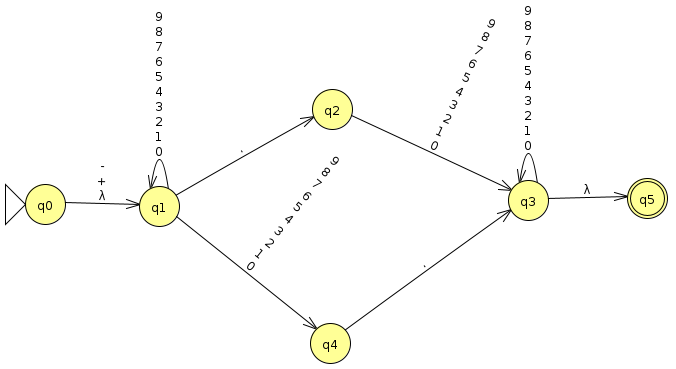
\includegraphics[scale=0.7]{e-NFA1.png}
				\end{center}
				Essendo lo stato \{q1,q4\} non raggiungibile, si omette nella tabella.\newline
				Formalmente, un $\varepsilon$-NFA E è definito come E=(Q,$\Sigma$,$\delta$,q0,F), dove l'unico parametro differente è la funzione di transizione, che prende in input uno stato in Q e un simbolo nell'alfabeto $\Sigma$$\cup$\{$\varepsilon$\}, restituendo un sottoinsieme di Q. \newline
				Essendo un particolare tipo di NFA, l'$\varepsilon$-NFA ha tutte le caratteristiche degli NFA.
		\subsection{DFA to NFA (e viceversa)}
			Sebbene possa sembrare controintuitivo, sia NFA che DFA riconoscono gli stessi linguaggi cambiando unicamente il metodo con cui li riconoscono.\newline Infatti, $\forall$ NFA N $\exists$ un DFA D : L(D)=L(N) (e viceversa). Per far ciò, si usa un metodo chiamato Costruzione a Sottoinsiemi.
			\subsubsection{Costruzione a Sottoinsiemi}
				La Costruzione a Sottoinsiemi ci permette, dato un NFA, di ricavare un DFA che possa riconoscere il linguaggio del NFA. In particolare, ogni stato del DFA corrisponde ad un insieme di stati del NFA, il DFA inizia in \{q0\}, ovvero nell'insieme di stati con solo q0, nel DFA una stato finale corrisponde ad almeno uno stato finale del NFA, e la funzione di transizione del DFA si riferisce ad uno stato contenuto nel target della funzione di transizione di un NFA.\newline \newline
				\textbf{Esempio} Prendiamo il seguente NFA:
				\begin{center}
					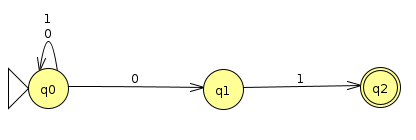
\includegraphics{NFADFA1.png}
				\end{center}
				Per "tradurlo" in un DFA, dobbiamo fare una tabella di "conversione", come la seguente:
				\begin{center}
					\begin{tabular}{c|c|c}
						&0&1 \\
						\hline
						$\rightarrow$ \{q0\} &\{q0,q1\}&\{q0\} \\
						\{q1\} &$\emptyset$&\{q2\}* \\
						\{q2\}* &$\emptyset$&$\emptyset$ \\
						\{q0,q1\} &\{q0,q1\}&\{q0,q1,q2\}* \\
						\{q0,q2\}* &\{q0,q1\}&\{q0,q1\} \\
						\{q1,q2\}*&$\emptyset$&\{q2\}*\\
						\{q0,q1,q2\}* &\{q0,q1\}&\{q0,q1,q2\}* 
					\end{tabular}
				\end{center}
				Ma se osserviamo, alcuni stati sono inutili, ovvero non contribuiscono in alcun modo alla creazione del DFA, e l'automa non passerà mai per quei stati. Se "puliamo" la tabella otteniamo:
				\begin{center}
					\begin{tabular}{c|c|c}
						&0&1 \\
						\hline
						$\rightarrow$ \{q0\} &\{q0,q1\}&\{q0\} \\
						\{q0,q1\} &\{q0,q1\}&\{q0,q1,q2\}* \\
						\{q0,q1,q2\}* &\{q0,q1\}&\{q0,q1,q2\}* 
					\end{tabular}
				\end{center}
				Che comprende gli stati che formano realmente il DFA. Se costruiamo il diagramma otteniamo:
				\begin{center}
					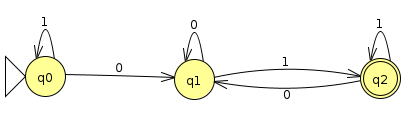
\includegraphics{NFADFA2.png}
				\end{center}
				Che è effettivamente corrispondente agli stati e alle transizioni della seconda tabella.\newline
				Tale operazione è possibile grazie ad un teorema, che ora enunciamo.
				\newline \newline
				\textbf{Teorema di equivalenza}\newline
				Un linguaggio L è accettato da un DFA $\Leftrightarrow$ L è accettato da un NFA
			\subsubsection{$\varepsilon$-chiusure}
				Nel caso di $\varepsilon$-NFA, si utilizza una versione modificata della costruzione a sottoinsiemi, caratterizzata dalle $\varepsilon$-chiusure. Con $\varepsilon$-chiusura s'intende l'eliminazione delle $\varepsilon$-transizioni dagli stati che ne fanno uso.\newline
				A livello pratico. la costruzione a sottoinsiemi è uguale a quella usata partendo da un NFA, con la variante che lo stato iniziale del DFA è dato dalle $\varepsilon$-chiusure dello stato iniziale del $\varepsilon$-NFA.
				\newline \newline
				\textbf{Esempio} Riprendiamo l'$\varepsilon$-NFA visto in precedenza:
				\begin{center}
					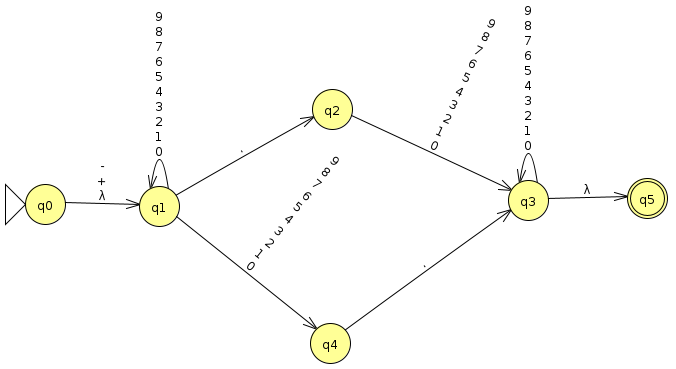
\includegraphics[scale=0.7]{e-NFA1.png}
				\end{center}
				Prima di effettuare la costruzione, dobbiamo effettuare le $\varepsilon$-chiusure: \newline \\
				ECLOSE(q0)=\{q0,q1\}\\
				ECLOSE(q1)=\{q1\}\\
				ECLOSE(q2)=\{q2\}\\
				ECLOSE(q3)=\{q3,q5\}\\
				ECLOSE(q4)=\{q4\}\\
				ECLOSE(q5)=\{q5\}\\
				Dopo questa operazione, possiamo applicare la costruzione. Riportiamo solo la tabella di transizione (per pigrizia):
				\begin{center}
					\begin{tabular}{c|c|c|c}
						&+,-&.&0,..,9 \\
						\hline
						$\rightarrow$ \{q0,q1\} &\{q1\}&\{q2\}&\{q1,q4\} \\
						\{q1\} &$\emptyset$&\{q2\}&\{q1,q4\} \\
						\{q2\} &$\emptyset$&$\emptyset$&\{q3,q5\}* \\
						\{q1,q4\} &$\emptyset$&\{q2,q3,q5\}&\{q1,q4\} \\
						\{q2,q3,q5\}* &$\emptyset$&$\emptyset$&\{q2.q3,q5\} \\
						\{q3,q5\}* &$\emptyset$&$\emptyset$&\{q3,q5\} \\
					\end{tabular}
				\end{center}
				Enunciamo anche il teorema per la conversione da $\varepsilon$-NFA a DFA:
				\newline
				\newline
				\textbf{Teorema}\newline
				Un linguaggio L è accettato da un DFA $\Leftrightarrow$ L è accettato da un $\varepsilon$-NFA
		\subsection{Espressioni Regolari}
			Abbiamo visto come un linguaggio regolare possa essere espresso tramite un automa a stati finiti. Però non è l'unico modo per descriverlo. Infatti, possiamo esprimerlo anche tramite un'espressione regolare, che non è altro che un modo dichiarativo per descrivere un linguaggio regolare.\\
			Gli ingredienti per costruire un'espressione regolare sono:\\
			-un'insieme di costanti: $\varepsilon$ indica la stringa vuota, $\emptyset$ indica il linguaggio vuoto e si usano i simboli presenti in un alfabeto $\Sigma$\\
			-operatori: + viene usato per l'unione, . viene usato per la concatenazione e * viene usato per la chiusura di Kleene (* include anche $\varepsilon$)\\
			-parentesi, per il raggruppamento\\\\
			Con L(E) si indica il linguaggio creato dall'espressione regolare. Essendo una dichiarazione del linguaggio, possono esserci più espressioni corrette per un linguaggio.\\\\
			\textbf{Esempio} Supponiamo di voler definire come espressione regolare il segeunte linguaggio:\\\\
			L=\{w $\in$ \{0,1\}* : 0 e 1 alternati in w\}\\\\
			Possiamo descriverlo in due modi: o come unione delle possibilità, cioè unione di una alternanza 01, 10, 10101 o 01010, oppure come alternanza di 01, ma con la possibilità di avere un 1 davanti o uno 0.\\
			Poniamolo come espressione, così che risulti più chiaro:\\\\
			\begin{center}
				(01)*+(10)*+1(01)*+0(10)*\\oppure\\ ($\varepsilon$+1)(01)*($\varepsilon$+0)
			\end{center}
			Si vede come, a livello pratico, non cambi nulla nel significato del linguaggio. Sta quindi a voi scegliere l'espressione che ritenete più opportuna.\\
			\textbf{Importante!} Esattamente come nel linguaggio naturale, le espressioni regolari sono soggette alle precedenze. In particolare, in assenza di parentesi ogni operatore si lega al simbolo alla sua sinistra. Quindi, per fare un esempio, una espressione del tipo 01*+1 viene raggruppata come (0(1)*)+1, e quindi è differente da (01)*+1.
		\subsection{Equivalenza tra FA e RE}
			Abbiamo quindi visto finora gli automi a stati finiti (DFA, NFA, $\varepsilon$-NFA) e le espressioni regolari. Ma sappiamo anche che entrambi i modi rappresentano un linguaggio. Tramite questa conoscenza, possiamo passare da un automa (un DFA) ad una espressione regolare e viceversa (ma il quel caso si passerà ad un $\varepsilon$-NFA, come vediamo a breve).
			\subsubsection{Da RE a $\varepsilon$-NFA}
				Il primo modo è passare da una espressione regolare ad una $\varepsilon$-NFA. Usiamo il seguente teorema:\\\\
				\textbf{Teorema} $\forall$ R espressione regolare possiamo costruire un $\varepsilon$-NFA A : L(A)=L(R)\\\\
				Per far sì che il $\varepsilon$-NFA riconosca il linguaggio dell'espressione regolare, bisogna costruire un $\varepsilon$-NFA tale che abbia un solo stato finale, non abbia alcuna transizione entrante nello stato iniziale e non abbia nessuna transizione uscente dallo stato finale. Di seguito le regole per rappresentare unione, concatenazione e chiusura di Kleene.
				\begin{center}
					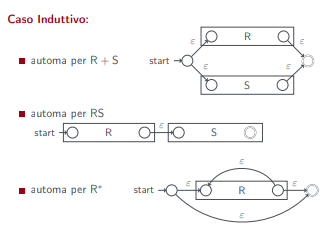
\includegraphics{ConversioneRENFA.png}
				\end{center}
				\textbf{Esempio} Consideriamo l'espressione regolare (0+1)*1(0+1).\\
				Notiamo che la prima unione è anche una chiusura di Kleene, quindi nel'automa per R*, il nostro R sarà l'automa che rappresenta l'unione 0+1. Seguirà una $\varepsilon$-transizione ad un automa che conti il primo carattere, il quale avrà un'altra $\varepsilon$-transizione al secondo automa che rappresenta l'unione 0+1. Di seguito riportiamo il diagramma di transizione per l'$\varepsilon$-NFA appena descritto.
				\begin{center}
					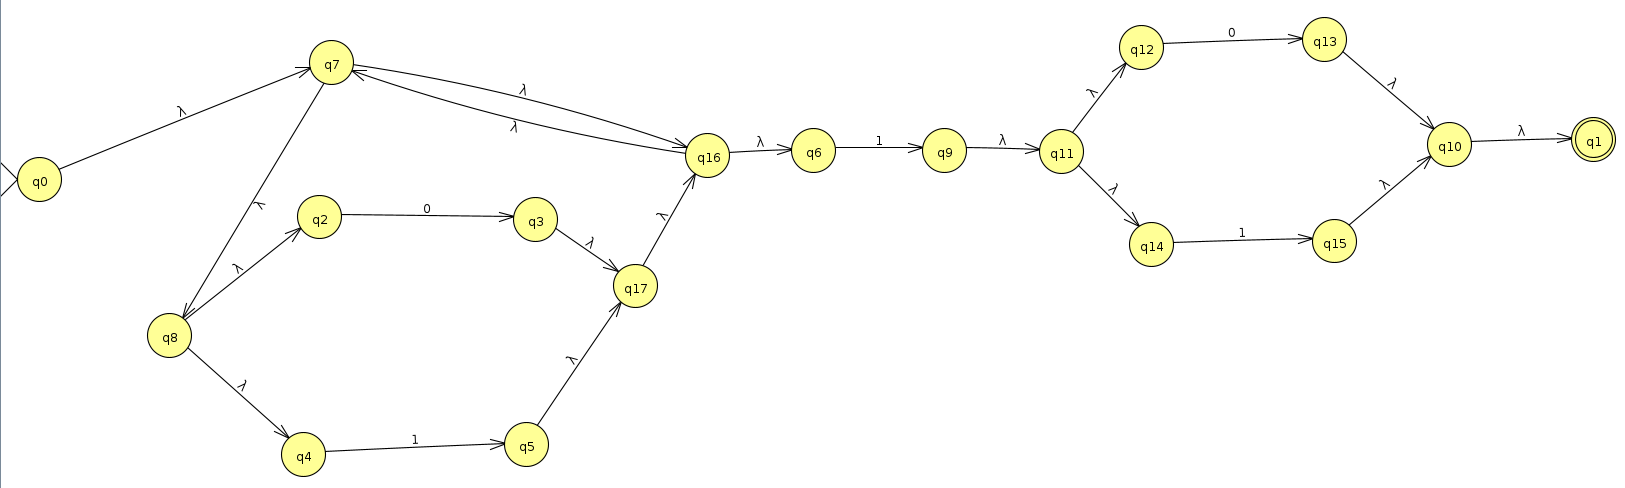
\includegraphics[scale=0.35]{RENFA1.png}
				\end{center}
				Notare che, fondamentalmente, si concatenano più pezzi di automi semplici tramite $\varepsilon$-transizioni.
			\subsubsection{Da DFA a RE}
				Se invece si ha un automa e si vuole passare ad una espressione regolare, si utilizza una tecnica chiamata \textbf{eliminazione di stati}.\\
				In pratica, quando uno stato viene eliminato, vengono eliminati anche i cammini per quello stato. Al suo posto, si mettono nuove transizioni con espressioni regolari, che descrivono anche le transizioni perse. Si continua finchè non si ha un'unica transizione, contenente il linguaggio riconosciuto dall'automa.\\
				Riassumendo, l'automa di partenza deve avere un unico stato finale (e in caso di più stati finali, se ne crea uno nuovo con $\varepsilon$-transizioni provenienti dai vecchi stati finali), s'iniziano a collassare le transizioni tra la stessa coppia di stati e si eliminano tutti gli stati tranne quello iniziale e quello finale. Se qr $\not$= q0, ovvero stato finale e stato iniziale sono distinti, allora l'automa ha 4 transazioni: R(che rimane in q0),S(che da q0 va in qr),U(che rimane in qr) e T(che da qr ritorna in q0). L'espressione regolare che lo descrive è (R+SU*T)*SU*. Nel caso q0=qr, l'automa ha un unico stato R e la sua espressione regolare è R*.\\
				\textbf{Esempio} Consideriamo il segeunte automa:\\
				\begin{center}
					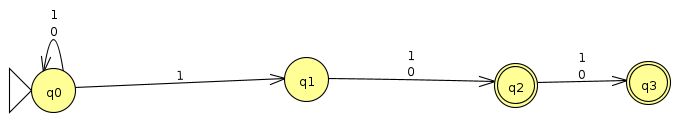
\includegraphics[scale=0.7]{DFARE1.png}
				\end{center}
				Guardando l'automa, possiamo già intuire che saremo nel caso in cui avremo q0 $\not$= qr. La prima operazione è creare uno stato q4, che sarà il nostro stato finale, essendoci 2 stati finali. Collassando le transizioni, otteniamo transizioni di unione, quindi nel nostro caso, in q0 per esempio, invece che una transizione per 0 ed una transizione per 1 otterremo un'unica transizione 0+1. Passando alla eliminazione degli stati, quando elimino q1 creo una transizione che va da q0 a q2, che in espressione regolare si esprime con 1(0+1), quando elimino q2 passo ad una transizione da q0 a q3 che vale 1(0+1)(0+1), mentre la transizione da q0 a q4, essendo 1(0+1) una transizione diretta, è 1(0+1)+1(0+1)(0+1).\\
				Quindi l'espressione regolare relativa all'automa visto è (0+1)*(1(0+1)+1(0+1)(0+1)).
		\subsection{Linguaggi non regolari}
			Finora abbiamo visto tutti i possibili modi per mostrare un linguaggio regolare, dall'automa all'espressione regolare. Ma prendiamo in esempio il seguente linguaggio:
			\begin{center}
				L01=\{0$^n$1$^n$ : n $\geq$ 0\}
			\end{center}
			Se un DFA con k stati legge 0$^k$, allora esiste un k+1 stato che è duplicato. Morale: se A legge 1$^i$ e finisce in uno stato finale, accetta la parola 0$^j$1$^i$, che non è nel linguaggio, mentre se finisce in uno stato non finale, rifiuta la parola 0$^i$1$^i$, che è nel linguaggio, ingannando in ogni caso l'automa. Tali linguaggi sono definiti non regolari.\\
			Il problema è che dire "Non riesco a costruirci un automa a stati finiti" non dice nulla, c'è bisogno di una prova oggettiva, che introduciamo con il teorema del Pumping Lemma.\\\\
			\textbf{Teorema} Supponiamo che L sia un linguaggio regolare. Allora $\exists$ una lunghezza k $\geq$ 0 tale che ogni parola w $\in$ L di lunghezza \textbar w\textbar $\geq$k può essere spezzata in w=xyz, tale che y $\not$= $\varepsilon$, \textbar xy\textbar $\leq$ k e $\forall$ i $\geq$ 0, xy$^i$z $\in$ L.\\\\
			Quindi, per dimostrare che un linguaggio non è regolare, si usa il Pumping Lemma assumendo L regolare, portandosi in questo modo in una condizione di assurdità (non sempre funziona, ma nella maggior parte dei casi).
	\section{Grammatiche di Linguaggi liberi da contesto e PDA}
		Passiamo ora ad una nuova parte, dove vedremo i inguaggi Context-Free.\\
		Questi linguaggi, a differenza dei linguaggi regolari e non, non  dipendono da un contesto, ma anche loro possono essere rappresentati in due modi, o come Grammatica Context-Free o come Automa a Pila, che vedremo successivamente.
		\subsection{Grammatiche Context-Free}
			Le Grammatiche Context-Free sono il primo modo per esprimere un linguaggio context-free. Esse utilizzano delle regole di sostituzione (generalmente hanno forme tipo A -\textgreater B), e queste regole possono avere variabili (tra cui una iniziale) o terminali (ovvero simboli dell'alfabeto che si utilizza).\\
			\textbf{Esempio} Vediamo la grammatica G1. Essa utilizza come alfabeto $\Sigma$=\{0,1,$\#$\} ed è composta da 3 regole:\\
			-A-\textgreater 0A1\\
			-A-\textgreater B\\
			-B-\textgreater $\#$\\
			Un esempio di parola è 000$\#$111.\\\\
			Come si vede nell'esempio, si parte dalla variabile iniziale (nell'esempio, A), e si segue la regola, finchè non rimangono solo i terminali. Generalmente queste regole sono espresse anche come alberi sintattici, come il seguente:
			\begin{center}
				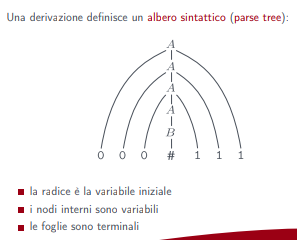
\includegraphics{TREE.png}
			\end{center}
			Formalmente, una grammatica context-free è definita come (V,$\Sigma$,R,S), dove V è un insieme finito di variabili, $\Sigma$ è un insieme finito di terminali disgiunto da V, R è un insieme di regole, S è la variabile iniziale (S $\in$ V).\\\\
			Ma come si progettano le grammatiche context-free? Fondamentalmente non esistono processi meccanici, però ci sono delle tecniche che possono tornare utili.\\
			La prima riguarda l'unione di linguaggi più semplici, essendo molti linguaggi l'unione di linguaggi più semplici. L'idea è di costruire grammatiche separate per ogni componente, per poi unire le due grammatiche con una nuova regola iniziale.\\
			La seconda, valida per i linguaggi regolari, consiste di prendere un DFA e trasformarlo in una grammatica context-free. L'idea sta nell'usare una variabile Ri per ogni stato qi, una regola ri -\textgreater aRj per ogni transizione e una regola Ri -\textgreater $\varepsilon$ per ogni stato finale qi. Se q0 è lo stato iniziale, la variabile iniziale è R0.\\
			La terza consiste nel vedere un linguaggio come formato da due sottostringhe collegate. L'idea in questo caso è usare regole nella forma R-\textgreater uRv, che generano stringhe dove u corrisponde a v.
			\subsubsection{Proprietà delle grammatiche context-free}
				Diamo la definizione di albero sintattico: data una grammatica G=(V,$\Sigma$,R,S), un albero sintattico è un albero i cui nodi interni sono variabili di V, le foglie sono simboli terminali o $\varepsilon$ e se un nodo interno è etichettato con A e i suoi figli sono, da sinistra a destra, X1,X2...Xk, allora A -\textgreater X1X2...Xk è una regola di G.\\
				Attenzione che un albero può generare una stringa in due modi diversi! Infatti, una grammatica genera ambiguamente una stringa se esistono due alberi sintattici diversi per quella stringa. Quindi, generalmente si effettua la derivazione a sinistra per evitare ambiguità.\\
				Diamo una definizione: una grammatica è definita ambigua se genera almeno una stringa ambiguamente.\\
				Inoltre esistono i linguaggi inerentemente ambigui, ovvero linguaggi che sono generati solo da grammatiche ambigue.\\
				Ora, una grammatica context-free è migliore se semplificata, ed una delle forme più semplici è la forma normale di Chomsky, che rende ogni regola della forma A-\textgreater BC, A-\textgreater a, dove a è un terminale, B e C non posssono essere la variabile iniziale.\\ Inoltre, può esserci la regola S -\textgreater $\varepsilon$ per la variabile iniziale S. Per trasformare una grammatica context-free in forma normale di Chomsky, si aggiunge una nuova variabile, si eliminano le $\varepsilon$-regole, si eliminano le regole unitarie A-\textgreater B e si trasformano le regole rimaste nella forma corretta appena vista.\\
				Segue un esempio, che non riporto a mano:\\
				\begin{center}
					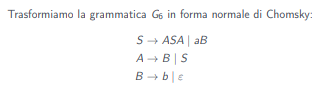
\includegraphics{CHOMSKY1.png}
					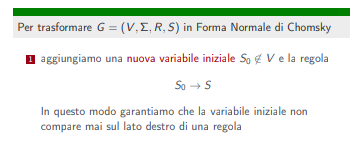
\includegraphics{CHOMSKY2.png}
					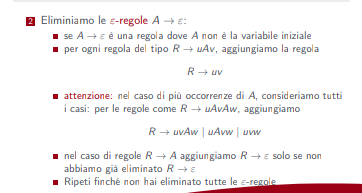
\includegraphics{CHOMSKY3.png}
					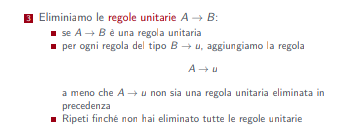
\includegraphics{CHOMSKY4.png}
					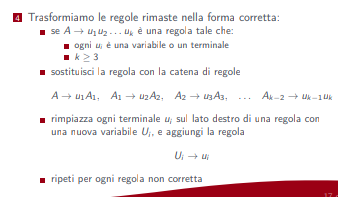
\includegraphics{CHOMSKY5.png}
				\end{center}
		\subsection{PDA}
			Gli automi a pila (dall'Inglese Pushdown Automation, abbreviato in PDA) sono degli automi che, oltre ad utilizzare gli stati, utilizzano anche una pila. La funzione di transizione stabilisce quali possono essere gli stati successivi e i simboli da scrivere nella pila, dati stato corrente, simbolo in input e il simbolo in cima alla pila. Inoltre, essendo la pila un tipo di memoria LIFO, permette all'automa di avere memoria infinita ad accesso limitato.\\
			Formalmente, un PDA viene definito come P=(Q,$\Sigma$,$\Gamma$,$\delta$,q0,F), dove Q è un insieme finito di stati, $\Sigma$ è l'alfabeto di input, $\Gamma$ è l'alfabeto della pila, $\delta$ è la funzione di transizione, q0 è lo stato iniziale e F è l'insieme di stati accettanti.\\
			\textbf{Esempio} Creiamo un PDA per il linguaggio L=\{0$^n$1$^n$ : n $\geq$ 0\}. Formalmente si definisce con P=(\{q0,q1,q2,q3\},\{0,1\},\{0,\$\},$\delta$,q0,\{q0,q3\}). Segue diagramma di transizione:
			\begin{center}
				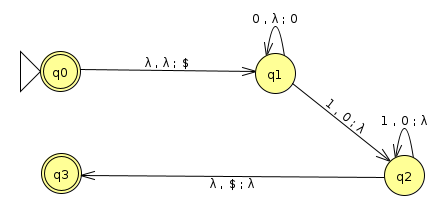
\includegraphics{PDA1.png}
			\end{center}
			L'esempio appena visto accetta una parola per stato finale, ma un PDA può accettare anche per pila vuota. Infatti, un PDA accetta la parola w per pila vuota se $\exists$ una computazione che consuma tutto l'input e termina con la pila vuota. Inoltre, $\forall$ linguaggio accettato da un PDA per stato finale $\exists$ un PDA che accetta per pila vuota, e viceversa.
		\subsection{Da Grammatiche Context-Free a PDA}
			Enunciamo subito un teorema, che ci farà notare una somiglianza tra gli automi a stati finiti e i PDA:\\
			\textbf{Teorema} Un linguaggio è context-free $\Leftrightarrow$ $\exists$ un PDA che lo riconosce\\
			L'idea è che P simula i passi di derivazione in G, e P accetta w se esiste una derivazione di w in G.\\
			La dimostrazione si fa creando un PDA P=(\{Qstart,Qloop,Qend\},$\Sigma$,$\Sigma$ $\cup$ V $\cup$ \{\$\},Qstart,{Qend}) e funzione di transizione $\varepsilon$,A-\textgreater u per la regola A-\textgreater u, a,a-\textgreater $\varepsilon$ per il terminale a (dove i vari stati sono presi dalla grammatica).
		\subsection{Da PDA a Grammatiche Context-Free}
			Per questo passaggio, andremo a fare una grammatica che fa un po' di più rispetto al PDA, ovvero generiamo una variabile Apq per ogni coppia di stati p,q di P, dove Apq genera ogni stringa che porta da p con pila vuota a q con pila vuota.\\
			Occorre però che il PDA da trasformare rispetti 3 condizioni, ovvero ha un unico stato accettante qf, svuota la pila prima di accettare, e ogni transizione effettua il push o il pop, ma non entrambe le azioni. In particolare, quest'ultima azione prevede due casi, la prima riguarda l'inserimento all'inizio e la rimozione alla fine, la seconda vede un inserimento all'inizio ma una rimozione prima della fine (in r, quindi invece che solo Apq, si avrà sia Apr che Arq).\\
			Formalmente, dato un PDA P=(Q,$\Sigma$,$\Gamma$,$\delta$,q0,\{qf\}), generiamo una grammatica G=(V,$\Sigma$,R,Aq0-qf) tale che\\
			V=\{Apq : p,q $\in$ Q\},\\ 
			$\forall$ p,q,r,s $\in$ Q, u $\in$ $\Gamma$ e a,b $\in$ $\Sigma$$\varepsilon$, se $\delta$(p,a,$\varepsilon$) contiene (r,u) e $\delta$(s,b,u) contiene (q,$\varepsilon$), aggiungiamo la regola Apq-\textgreater aArsb, \\
			$\forall$ p,q,r $\in$ Q, aggiungiamo la regola Apq-\textgreater AprArq,\\
			$\forall$ p $\in$ Q, aggiungiamo la regola App-\textgreater $\varepsilon$.
		\subsection{Linguaggi non context-free}
			Abbiamo visto, per i linguaggi regolari, che il Pumping Lemma è il modo per dimostrarne la regolarità. Similmente, esiste il Pumping Lemma per linguaggi context-free, di cui ora diamo l'enunciato.\\\\
			\textbf{Teorema} Sia L un linguaggio context-free. Allora $\exists$ una lunghezza k $\geq$ 0 tale che $\forall$ w $\in$ L di lunghezza \textbar w\textbar $\geq$ k può essere spezzata in w=uvxyz tale che \textbar vy\textbar \textgreater 0, \textbar vxy\textbar $\leq$ k, $\forall$ i $\geq$ 0, uv$^i$xy$^i$z $\in$ L.\\\\
			L'unica differenza, rispetto ai linguaggi regolari, è che in questo caso la parola viene divisa in 5 parti, e le parti "pompate" sono 2. Questo perché, per i linguaggi context-free, si replica il sottoalbero (ripetuto) di R rimanendo nel lingauggio (a parità di w "molto lunga" e albero sintattico relativo "molto alto"). Di seguito una dimostrazione grafica.
			\begin{center}
				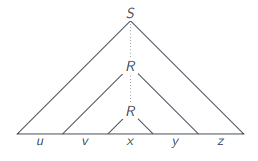
\includegraphics{PLCFG1.png}
				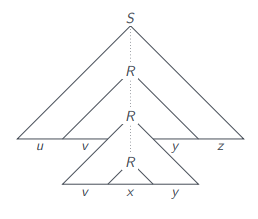
\includegraphics{PLCFG2.png}
				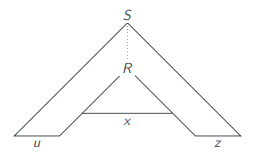
\includegraphics{PLCFG3.png}
			\end{center}
			Includiamo inoltre proprietà degli alberi e dimostrazione, sempre in forma grafica.
			\begin{center}
				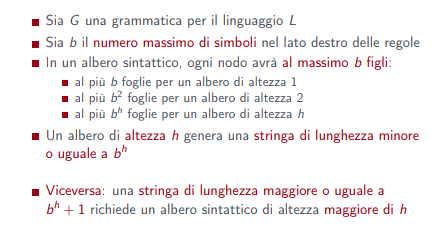
\includegraphics{PLCFG4.png}
				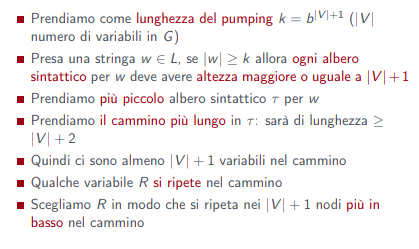
\includegraphics{PLCFG5.png}
				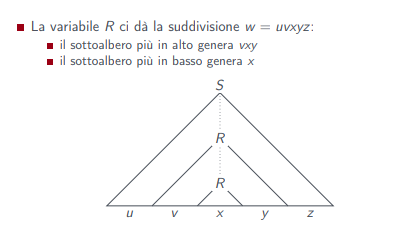
\includegraphics{PLCFG6.png}
				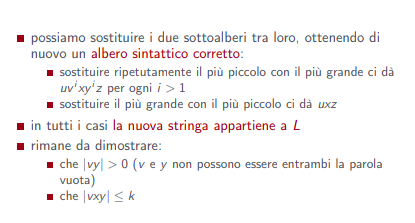
\includegraphics{PLCFG7.png}
				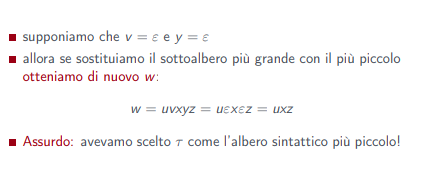
\includegraphics{PLCFG8.png}
				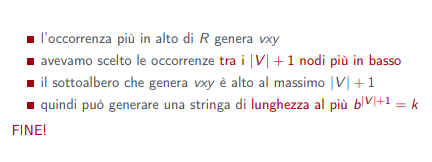
\includegraphics{PLCFG9.png}
			\end{center}
	\section{Decidibilità e macchine di Turing}
		Finora si sono visti sia automi a stati finiti (DFA, NFA, $\varepsilon$-NFA), sia automi a pila (PDA). Questi modelli hanno però una memoria limitata, o accessibile per un numero finito di volte. In questa sezione, vedremo un nuovo modello di automi, chiamati Macchine di Turing.
		\subsection{Macchine di Turing}
			Le Macchine di Turing (dall'inglese Turing Machines, abbreviato TM) altro non sono che un modello di calcolo proposto da (indovinate?) Alan Turing, nel 1936.\\\\ Tali macchine hanno una memoria illimitata e senza restrizioni, fondamentalmente rappresenta ogni calcolo che un computer reale può fare. Da ciò se ne deduce che se una TM non può risolvere un determinato problema, tale problema non può essere risolto da un computer poichè ne supera le capacità.\\\\
			Si è detto che una TM ha memoria infinita e con accesso illimitato. Infatti, la memoria è rappresentata da un nastro infinito, con inizialmente l'input scritto su esso, dove una testina ci legge e ci scrive i simboli. Tale testina può muoversi in qualunque direzione, e legge stati speciali sia per l'accettazione che per il rifiuto di una parola, che hanno effetto immediato. Formalmente, si definisce in questo modo una TM:\\\\
			M=(Q,$\Sigma$,$\Gamma$,$\delta$,q0,qAccept,qReject), dove Q è l'insieme finito di stati, $\Sigma$ è l'alfabeto di input e non contiene ␣ , $\Gamma$ è l'alfabeto del nastro, contiene sia il simbolo di blanck che i simboli presenti in $\Sigma$, $\delta$ è la funzione di transizione Q x $\Gamma$ $\mapsto$ Q x $\Gamma$ x \{L,R\}, q0 è lo stato iniziale, qAccept è lo stato accettante e qReject è lo stato di rifiuto, diverso da qAccept (ovviamente q0,qAccept,qReject $\in$ Q).\\\\
			Inoltre, una TM viene descritta da una configurazione, ovvero una tripla uqv, dove q è lo stato corrente, u è il contenuto del nastro prima della testina e v è il contenuto del nastro dalla testina in poi. La testina è posizionata sul primo simbolo di v. Una configurazione C1 produce C2 se la TM in questione, in un passo, passa da C1 a C2.\\
			\textbf{Esempio} Prendiamo in esame a,b,c $\in$ $\Gamma$ e u,v $\in$ $\Gamma^*$, con qi,qj stati. Allora:\\
			Se $\delta$(qi,b)=(qj,c,L), la configurazione uaq$_i$bv produce uq$_j$acv,\\
			se $\delta$(qi,b)=(qj,c,R), la configurazione uaq$_i$bv produce uacq$_j$v.ì\\\\
			Per quanto riguarda le fasi iniziali e finali, q0w è la configurazione iniziale (con w l'input), una configurazione con stato qAccept è una configurazione di accettazione e una configurazione con stato qReject è una configurazione di rifiuto. Le configurazioni di accettazione e di rifiuto sono configurazioni di arresto.\\\\
			Introduciamo ora i concetti di linguaggi Turing-riconoscibili e linguaggi Turing-decidibili. Un linguaggio è \textbf{Turing-riconoscibile} se $\exists$ una TM che lo riconosce, ovvero $\forall$ i,j=1,...,k C1 è la configurazione iniziale, ogni Ci produce Ci+1 e la configurazione di accettazione è Ck.\\ Un linguaggio è invece \textbf{Turing-decidibile} se $\exists$ una TM che lo decide, ovvero se dando un input M alla TM, essa termina sempre la computazione.\\\\
			\textbf{Esempio} Introduciamo un esempio di TM. Supponiamo di avere il seguente linguaggio:
			\begin{center}
				A=\{$0^{2^n}$ : n $\geq$ 0\}
			\end{center}
			Tale linguaggio ha una TM che decide il linguaggio A. In particolare, scorre il nastro da sinistra a destra, cancellando ogni secondo 0. Se il nastro conteneva un solo 0, accetta. Se invece il nastro conteneva un numero dispari di 0, rifiuta. Tale operazioni sono ripetute nel caso non si verifichino i due casi precedenti.
			\subsubsection{Varianti}
				Oltre alla definizione che abbiamo appena osservato, esistono delle definizioni differenti di TM, che chiameremo varianti.\\
				La prima è la \textbf{TM a nastro semi-infinito}, dove la testina è posizionata all'inizio del nastro e la testina è infinita solo verso destra. Ovviamente la testina può muoversi esattamente come in una TM classica, con l'unica eccezione che se richiede uno spostamento a sinistra a inizio nastro, la testina non si muove. Segue il teorema:\\\\
				\textbf{Teorema}: $\forall$ TM a nastro semi-infinito $\exists$ una TM a nastro infinito equivalente (e viceversa).\\\\
				Seguono ora le \textbf{TM multinastro}, dove una TM ha k nastri semi-infiniti. Logicamente, utilizza anche k testine per la lettura e la scrittura dei nastri. Il funzionamento differisce leggermente, poichè l'input per la TM si trova sul primo nastro, e ad ogni passo scrive e si muove simultaneamente su tutti i nastri. Prima di introdurre il teorema, dobbiamo parlare della sua funzione di transizione:\\\\
				$\delta$: Q x $\Gamma^k$ $\rightarrow$ Q x $\Gamma^k$ x \{L,R\}$^2$\\\\
				Se lo stato è qi e le testine leggono a1,...,ak allora scriviamo b1,...,bk sui k nastri, e poi muovendo ogni testina a sinistra o destra come specificato.\\\\
				\textbf{Teorema}: $\forall$ TM multinastro $\exists$ una TM a singolo nastro equivalente.\\
				L'idea è di creare una TM dove il nastro è formato dai k nastri, separati dal carattere \#, e indicando con un punto la posizione della testina.\\\\
				Possiamo anche definire un \textbf{Corollario}: Un linguaggio è Turing-riconoscibile $\Leftrightarrow$ $\exists$ una TM multinastro che lo riconosce.\\
				Tale corollario è valido poichè abbiamo definito una TM multinastro come una variante di una TM regolare.\\\\
				Passiamo ora alle \textbf{TM non deterministiche}, dove sono possibili più strade durante la computazione. Per semplicità considereremo delle TM a nastro semi-infinito. Per queste TM, la computazione è un albero decisionale, e la TM accetta se $\exists$ un ramo che porta allo stato accettante. Anche in questo caso abbiamo bisogno di una nuova funzione di transizione:\\\\
				$\delta$: Q x $\Gamma$ $\rightarrow$ 2$^{(Qx \Gamma x\{L,R\})}$\\\\
				Quindi questa computazione richiede l'esaminazione di ogni ramo, fino a quello di accettazione (se esiste). Segue il teorema:\\\\
				\textbf{Teorema}: $\forall$ TM non deterministica $\exists$ una TM deterministica equivalente.\\
				In queste TM, il terzo nastro (in una TM a 3 nastri) tiene traccia delle scelte non deterministiche.\\\\
				Anche con queste TM possiamo definire un \textbf{Corollario}: Un linguaggio è Turing-riconoscibile $\Leftrightarrow$ $\exists$ una TM non deterministica che lo riconosce. Anche in questo caso, una TM non determinista può essere trasformata in una TM deterministica, rendendo valido il corollario.\\\\
				Vediamo ora gli \textbf{Enumeratori}, ovvero TM che usufruiscono anche di una stampante. Un linguaggio è detto enumerato se ne ha stampato tutte le stringhe, sono ammesse ripetizioni.\\
				Ne segue subito il \textbf{Corollario}: Un linguaggio è Turing-riconoscibile $\Leftrightarrow$ $\exists$ un enumeratore che lo enumera.\\\\
				Concludiamo con le \textbf{TM monodirezionali}, dove la macchina non può spostare la sua testina a sinistra, ma può tenerla ferma o spostarla a destra. Funzione di transizione: $\delta$: Q x $\Gamma$ $\rightarrow$ Q x $\Gamma$\{S,R\}.\\\\
				Esistono poi altri modelli, che non affrontiamo. Quel che è rilevante sono gli elementi in comune, ovvero l'accesso senza restrinzioni ad una memoria illimitata, e l'equivalenza tra i vari modelli.
			\subsubsection{Algoritmi}
				Parliamo ora degli algoritmi per le TM. O meglio, di come possiamo descrivere la procedura con cui una TM riconosce, o decide, un determinato linguaggio.\\
				Essenzialmente esistono 3 modi: la descrizione formale, la descrizione implementativa e la descrizione di alto livello.\\
				Nella \textbf{descrizione formale} ogni singolo elemento è descritto in maniera dettagliata, e tutto è dichiarato esplicitamente. Questo metodo è sconsigliato poichè alle volte non è possibile descrive tutto dettagliatamente, ed è da evitare il più possibile.\\
				Nella \textbf{descrizione implementativa} non vengono espressi dettagli sugli stati, e vengono espressi a parole il movimento della testina e la scrittura sul nastro. Questa descrizione è più tollerata rispetto alla precedente, ma non è la descrizione ottimale.\\
				Nella \textbf{descrizione ad alto livello}, l'algoritmo viene descritto a parole e non viene fornito alcun dettaglio implementativo. Questa descrizione è quella da preferire sempre, tranne quando specificato di usarne una diversa.\\
				Segue un esempio:
				\begin{center}
					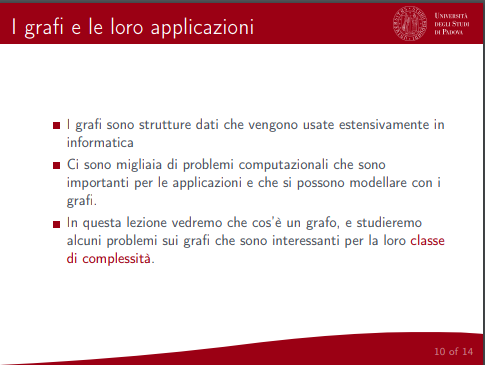
\includegraphics[scale=0.8]{algoritmo1.png}
					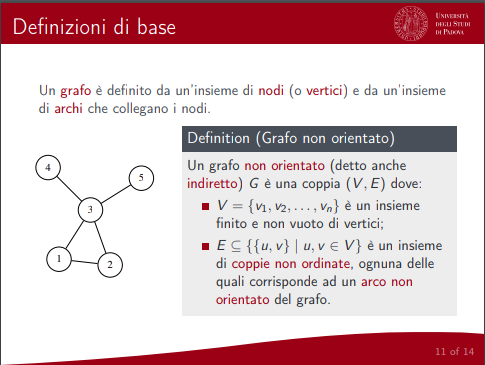
\includegraphics[scale=0.8]{algoritmo2.png}
					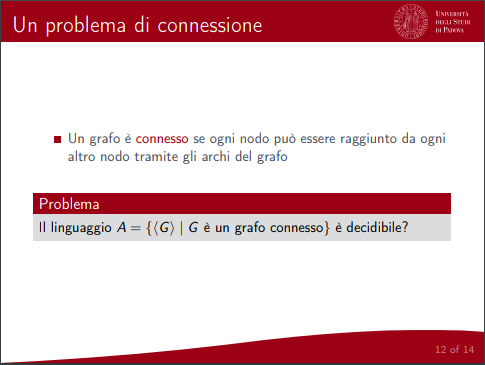
\includegraphics[scale=0.8]{algoritmo3.png}
					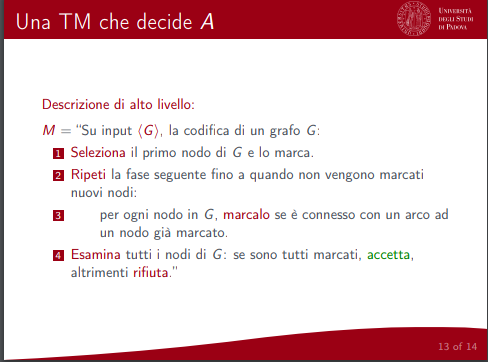
\includegraphics[scale=0.8]{algoritmo4.png}
					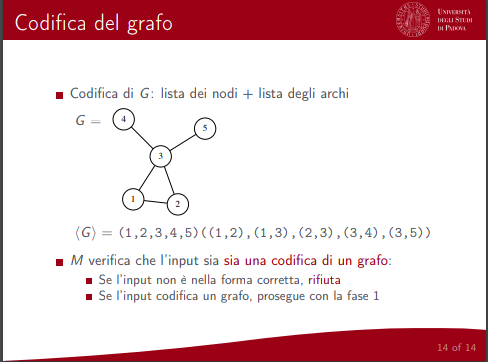
\includegraphics[scale=0.8]{algoritmo5.png}
				\end{center}
		\subsection{Linguaggi decidibili}
			In questa sezione, si tratteranno quali sono i linguaggi decidibili, ovvero se i linguaggi sono risolvibili o meno mediante un algoritmo.\\
			Iniziamo vedendo i \textbf{problemi sui linguaggi regolari}. Una TM converta un DFA, un NFA o una RE in un'altra codifica. L'importante è mostrare che il linguaggio è decidibile mostrando che il problema computazione è decidibile. Di seguito alcuni esempi:
			\begin{center}
				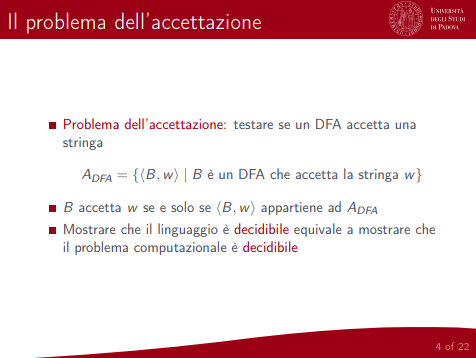
\includegraphics[scale=0.8]{problemaRegolare1.png}
				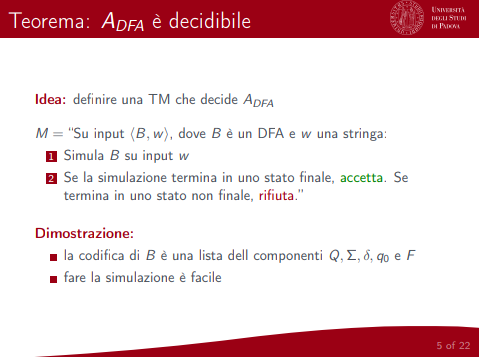
\includegraphics[scale=0.8]{problemaRegolare2.png}
				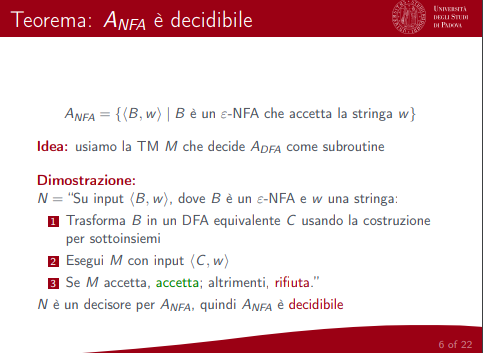
\includegraphics[scale=0.8]{problemaRegolare3.png}
				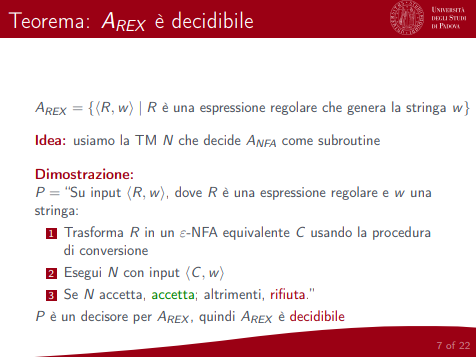
\includegraphics[scale=0.8]{problemaRegolare4.png}
				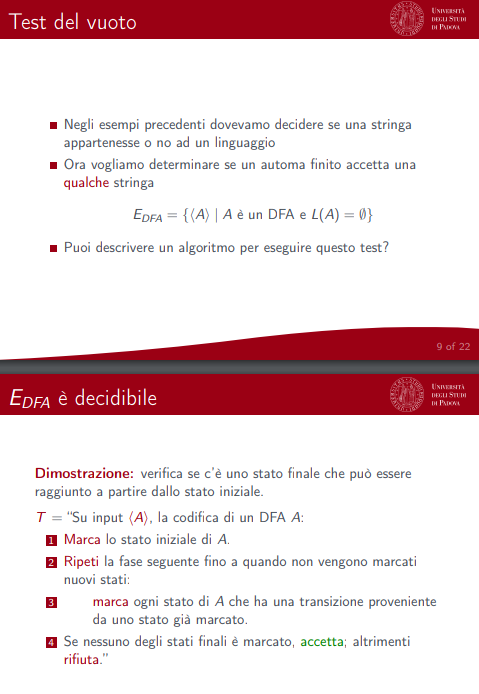
\includegraphics[scale=0.8]{problemaRegolare5.png}
				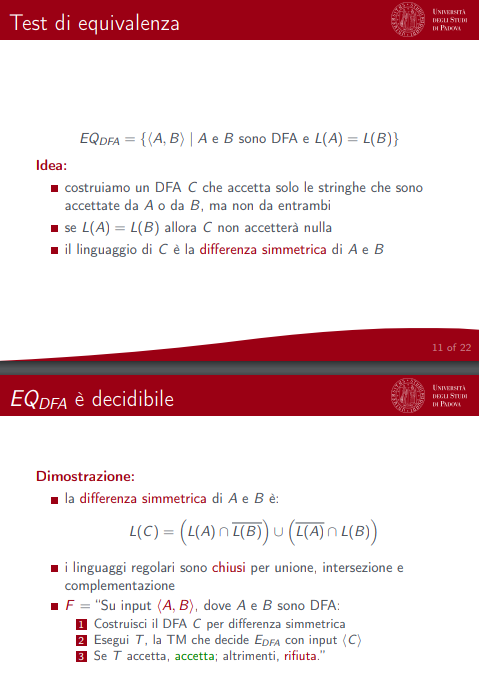
\includegraphics[scale=0.8]{problemaRegolare6.png}
			\end{center}
			Vediamo ora i \textbf{problemi sui linguaggi Context-free}, mostrando direttamente gli esempi:
			\begin{center}
				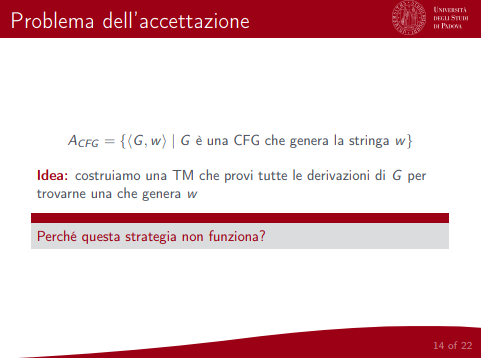
\includegraphics[scale=0.8]{problemaCF1.png}
				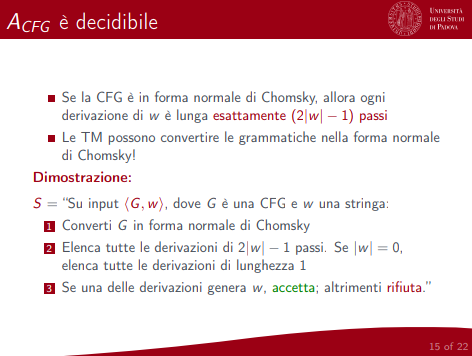
\includegraphics[scale=0.8]{problemaCF2.png}
				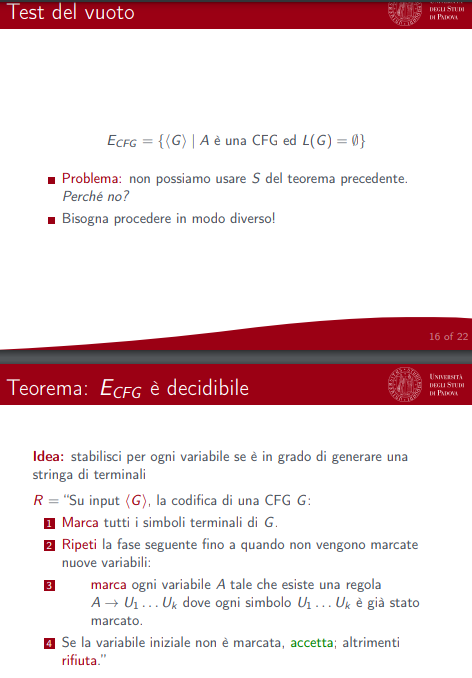
\includegraphics[scale=0.8]{problemaCF3.png}
				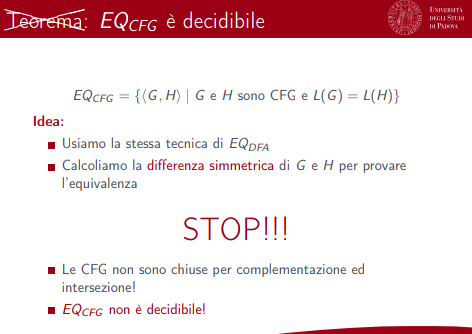
\includegraphics[scale=0.8]{problemaCF4.png}
			\end{center}
			Concludiamo dando la relazione tra le classi di linguaggi:\\\\
			Regolari $\subseteq$ Context-free $\subseteq$ Decidibili $\subseteq$ Turing-riconoscibili\\\\
			Queste non sono solo classi di linguaggi, ma anche classi di capacità computazionale.
		\subsection{Indecidibilità e riducibilità}
			Ora passiamo alla indecidibilità e riducibilità di un algoritmo, ovvero come dimostrare se un algoritmo è indecidibile, ovvero non può essere risolto algoritmicamente, e un metodo per la dimostrazione, ovvero la riducibilità.
			\subsubsection{Indecidibilità}
				Essendo quasi tutto legato ad esempi, si riportano le immagini.
				\begin{center}
					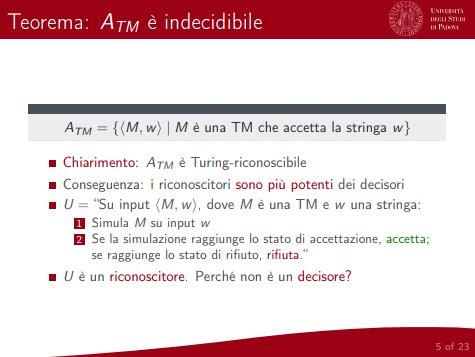
\includegraphics[scale=0.8]{indecidibile1.png}
					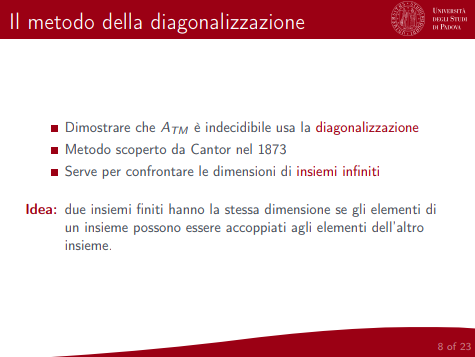
\includegraphics[scale=0.8]{indecidibile2.png}
					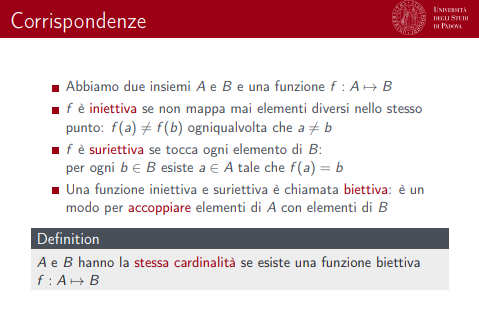
\includegraphics[scale=0.8]{indecidibile3.png}
					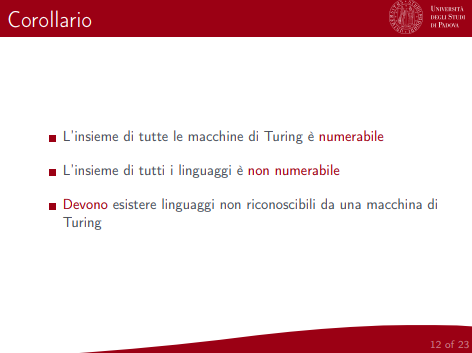
\includegraphics[scale=0.8]{indecidibile4.png}
					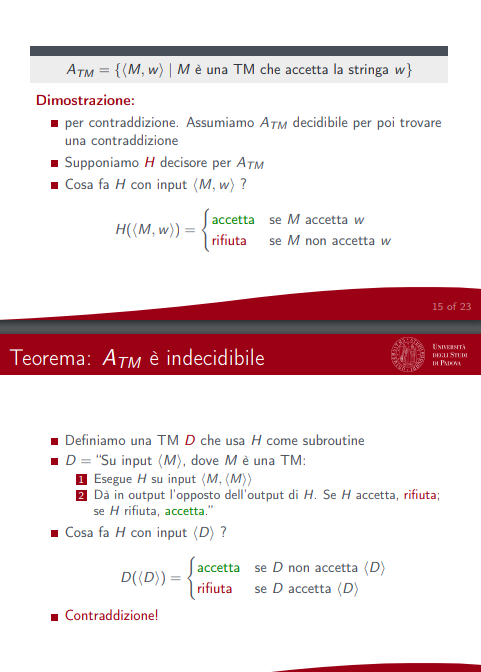
\includegraphics[scale=0.8]{indecidibile5.png}
					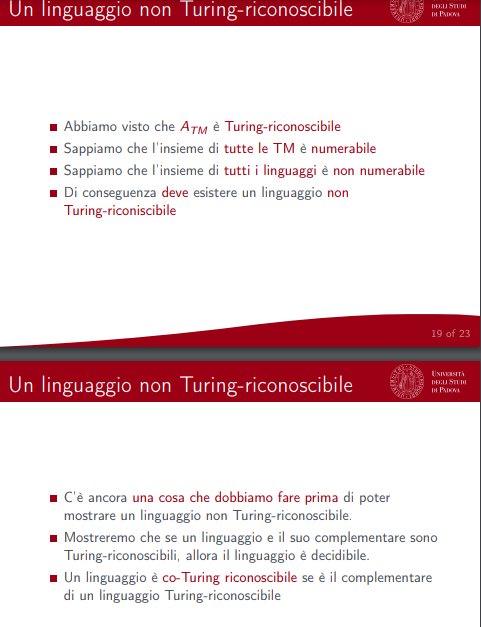
\includegraphics[scale=0.8]{indecidibile6.png}
					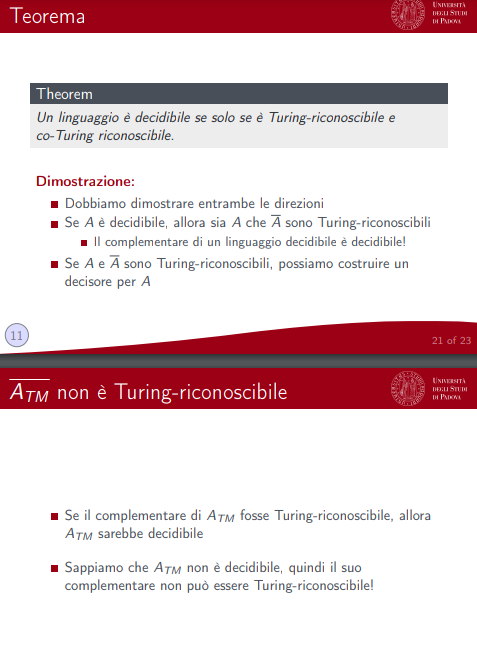
\includegraphics[scale=0.8]{indecidibile7.png}
				\end{center}
			\subsubsection{Riducibilità}
				La riduzione permette la trasformazione di un problema di un altro problema, di cui si può ricavare la soluzione, in modo da risolvere il problema originale.\\
				In tal modo, prendendo A e B due problemi distinti, se A è riducibile a B e B è decidibile, allora anche A è decidibile. Mentre, se A è riducibile a B e A è indecidibile, allora pure B è indecidibile.\\
				Tale riduzione può avvenire anche mediante una funzione. Seguono rappresentazione grafica e relativi esercizi/teoremi.
				\begin{center}
					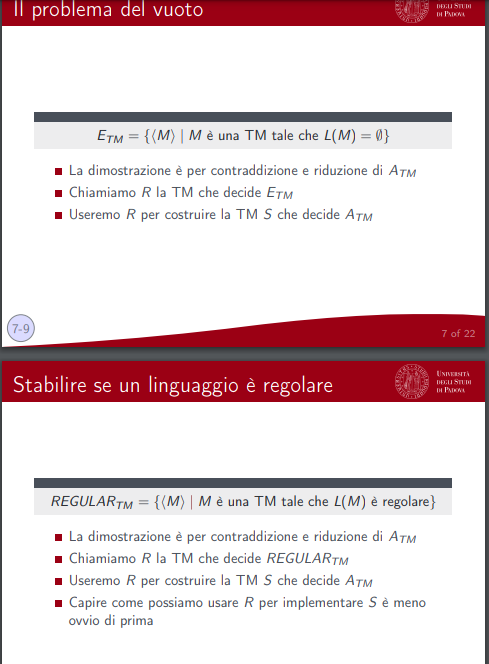
\includegraphics[scale=0.8]{riducibile1.png}
					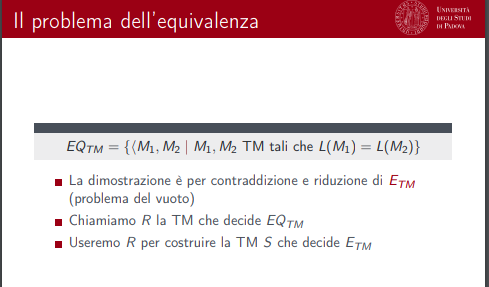
\includegraphics[scale=0.8]{riducibile2.png}
					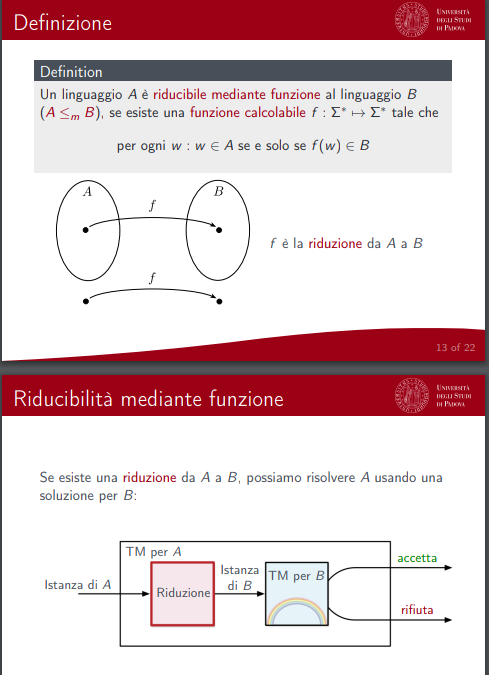
\includegraphics[scale=0.8]{riducibile3.png}
					\includegraphics[scale=0.8]{riducibile4.png}
					\includegraphics[scale=0.8]{riducibile5.png}
				\end{center}
	\section{Teoria della complessità}
		\subsection{Complessità di tempo}
		\subsection{Tempo Polinomiale}
		\subsection{La classe NP}
		\subsection{Problemi NP completi}
	\section{Esercizi svolti}
		\includepdf{Esempi di esame - Testi e soluzioni (1)/2106017_prima_parte_soluzione.pdf}
		\includepdf[pages=-]{Tutorato/01TutoratoSol.pdf}
		\includepdf[pages=-]{Tutorato/02SolTutorato.pdf}
		\includepdf[pages=-]{Tutorato/03SolTutorato.pdf}
		\includepdf[pages=-]{Tutorato/04SolTutorato.pdf}
		\includepdf[pages=-]{Tutorato/05SolTutorato.pdf}
\end{document}
